\begin{wrapfigure}[0]{r}[11pt]{0cm}
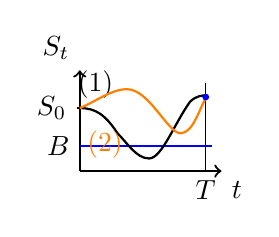
\begin{tikzpicture}[scale=0.4]
    % --- 定义参数 ---
    \def\T{4}         % 时间 T 的 x 坐标
    \def\Szero{2.0}   % S0 的 y 坐标
    \def\B{0.8}       % Barrier B 的 y 坐标 (蓝色线)

    % --- 绘制坐标轴 ---
    \draw[->, thick] (0, 0) -- (\T + 0.5, 0) node[below right] {$t$};
    \draw[->, thick] (0, 0) -- (0, 3.2) node[above left] {$S_t$};

    % --- 绘制辅助线和标签 ---
    % 蓝色障碍线 B
    \draw[blue, thick] (0, \B) node[left, black] {$B$} -- (\T + 0.2, \B);
    
    % S0 标记
    \draw[thick] (-0.1, \Szero) node[left] {$S_0$} -- (0.1, \Szero);
    
    % T 时刻竖线
    \draw[thin] (\T, 0) node[below] {$T$} -- (\T, 2.8);

    % --- 绘制路径 ---
    
    % 路径 1 (黑色): 下穿障碍线 B，再回升
    % 使用贝塞尔曲线模拟手绘的随机波动
    \draw[thick, black] (0, \Szero) 
        .. controls (0.5, \Szero) and (0.8, 1.8) .. (1.2, 1.2) % 下降段
        .. controls (1.5, 0.9) and (1.8, 0.4) .. (2.2, 0.4)    % 穿过 B 线，到达底部
        .. controls (2.6, 0.4) and (3.0, 1.5) .. (3.5, 2.2)    % 回升
        .. controls (3.7, 2.4) and (3.9, 2.4) .. (\T, 2.4);    % 终点
    
    % 路径 1 的标号 ①
    \node[above] at (0.5, \Szero) {(1)};

    % 路径 2 (橙色): 保持在上方，或者波动较平缓
    \draw[thick, orange] (0, \Szero)
        .. controls (0.5, 2.2) and (1.0, 2.6) .. (1.5, 2.6)    % 上升段
        .. controls (2.2, 2.6) and (2.8, 1.2) .. (3.2, 1.2)    % 下降但不穿过 B
        .. controls (3.6, 1.2) and (3.8, 2.0) .. (\T, 2.3);    % 回升至终点附近

    % 路径 2 的标号 ②
    \node[orange, below] at (0.8, 1.6) {(2)};

    % --- 终点的小圆圈 (蓝色涂鸦) ---
    \draw[blue, thick] (\T, 2.35) circle (2pt);
    % 模拟手绘的稍微杂乱的圆圈效果
    \draw[blue, thin] (\T, 2.35) circle (1.5pt);

\end{tikzpicture}
\end{wrapfigure}